% Kelompok 1 Tugas 3 GIS (Home)
% Mohammad Arya Rosyd Sikumbang (1154075)
% Ariana Setiawan (1154042)
% Arya Niken Manalu (1154080)
% Idang Mawardi (1154084)
% R Rifa Fauzi Komara (1154089)
% Andi Tentri Wali (1154013)

\section{Home}
	Pemrograman python adalah bahasa pemrograman terpopuler di tahun 2016 menurut tiobe. Python juga memiliki sintak atau aturan penulisan code pemrograman. Salah satu bagian Home merupakan halaman pengantar untuk mempelajari python . sebelum ketahapan yang baru selain home ini pembaca memerlukan pengertian yang lain yaitu seperti enverinmoment setup, syntax dan lain lain, awal untuk penulis jelakan yaitu pengertian tentang class pada python untuk mengantarkan logika dan pengetahuan apa itu class.
	Bahasa Pemrograman Python sudah dirasakan cukup matang untuk memecahkan masalah dalam dunia komputasi dan pengembangan sistem informasi. Manajemen paket Red Hat Linux, Blender,  PyGame, ZOPE (Framework Python untuk web services) telah membuktikan kepada kita semua bahwa Python merupakan bahasa pemrograman yang perlu diajarkan pada perguruan tinggi, terutama konsep interpreter, object oriented programming dan lainnya.
	Phyton dapat berjalan dibanyak platform atau sistem operasi seperti windows, linux/unix, mac OS X, OS/2, amiga, palm handhelds dan telepon genggam nokia. namun saat ini python juga sudah masuk kedalam virtual java dan NET. Python memiliki beberapa keunggulan, yaitu :
\begin{enumerate}
\item Syntaxnya sangat bersih dan mudah dibaca
\item Kemampuan melakukan pengekan syntaxnya yang kuat
\item Berorientasi objek secara intuisif
\item Kode-kode prosedure dinyatakan pada ekspresi natural
\item Modularitas yang penuh, mendukung hirarki paket
\item Penanganan error dilakukan berdasar pada eksepsi
\item Tipe-tipe data dinamis berada pada tingkat sangat tinggi
\item Library standar dapat diperluas dan modul dari pihak ketiga dapat dibuat secara virtual untuk setiap kebutuhan
\item Ekstensi dan modul-modul dapat secara mudah ditulis dalam C, C+ (atau java untuk Jython atau NET untuk IronPytho)
\item Dapat dimasukan kedalam aplikasi sebagai antar muka skrip
\end{enumerate}

\subsection{Kenapa alasan memilih Pemograman Phyton}
\begin{enumerate}
\item Python memiliki konsep desain yang bagus dan sederhana, yang berfokus pada kemudahan dalam penggunaan. Kode Python dirancang untuk mudah dibaca, dipelajari, digunakan ulang, dan dirawat. Selain itu, Python juga mendukung pemograman berorientasi objek dan pemograman fungsional.
\item Python dapat meningkatkan produktivias dan menghemat waktu bagi para programmer.Untuk memperoleh hasil program yang sama, kode Python juga jauh lebih sedikit dibandngkan dengan kode yang ditulis menggunakan bahasa-bahasa pemograman lain seperti C, C++,C# maupun Java. Coba lihat ilustrasi gambar dibawah ini:Bagaimana menurut kamu ? Sudah pasti Pyhton lebih sederhana dibanding bahasa-bahasa pemograman lain.
\item Program yang ditulis menggunakan Python ,dapat dijalankan di hampir semua sistem operasi (Unix, Windows, Mac OS X, dll), termasuk untuk perangkat-perangkat mobile.
\item Python memiliki banyak dukungan pustaka yang dikembangakan oleh pihak ketiga, misalnya pustaka untuk pengembangan web, pengembangan aplikasi visual (berbasis GUI), pengembangan permainan komputer (game), dan masih banyak lagi yang lainnya.
\item Melalui mekanisme tertenu, kode Python dapat diintegrasikan dengan aplikasi yang ditulis dalam bahasa pemograman lain. Sebagai contoh, kode Python dapat dipanggil dari kode C/C++, dan begitu juga perkembangan .NET Framework.
\item Terakhir, Python bersifat gratis atau bebas (free) dan open source, meskipun digunakan untuk kepentingan komersial.
\end{enumerate}

\subsection{Ranah Aplikasi Python}
Python dapat digunakan untuk membangun aplikasi-aplikasi berjalan pada banyak fungsi. diantaranya adalah sebagai berikut :
\begin{enumerate}
\item Pengembangan web dan internet. Dimana python mampu mengembangkan web dan internet seperti : penulisan skrip Common Gateway Internet (CGI), pengembangan frameworks seperti djago dan turbo gears, python juga mendukung penuh HTML, dan XML, pemrosesan e-mail, pemrosesan RRS feeds dll.
\item Akses terhadap database. antar muka open database connectivity (ODBC) untuk MySQL, Oracle,postgreSQL, SybaseODBC. dan juga mampu menyediakan Appication Programming Interface (API)
\item Pengembangan Graphical User Interface (GUI) pada Dekstop
\item Keperluan perhitung scientific dan numeris.
\item Pengembangan perangkat lunak komputer.
\item Pengembangan jaringan komputer.
\end{enumerate}

\subsection{interpreter python}
Bahasa pemrograman pyhton dilengkapi dengan suatu fasilitas seperti shell di linux, yang digunakan secara berulang dikemudian hari. untuk keperluan pernulisan ekspresi kompleks, kita dapat membuatnya dalam sebuah script yang dibantu dengan adanya teks editor. berikut adalah contoh dari statement dasar, perulangan dan seleksi :

\subsubsection{perulangan}
Dimana pada python dalam perulangan menggunakan statement for dan while. Yang dimana memiliki ciri berupa insialiasi perulangan dilakukan diawal statement dan perulangan itu akan berhenti bila syarat atua kondisi yang telah ditemukan terpenuhi.
Beberapa bentuk while adalah sebagai berikut :
Perulangan sederhana 
while x < 10: 
  print x, 
  $x = x + 1$ 
Perulangan di dalam perulangan 
while x < 10: 
  while y < 10: 
    print y,  
     $y = y + 1$ 
    print x, 
    $x = x + 1$
 Perulangan yang terus menerus
 while 1: 
    print \‘selamanya mengulang\’ 
  Perulangan dengan else 
  while x < 10: 
    print x, 
    $x = x + 1$ 
   else: 
    print \‘Perulangan sudah selesai\’ 
   Hasilnya : 
   Python 2.4.3 (#1, May 24 2008, 13:47:28) 
   [GCC 4.1.2 20070626 (Red Hat 4.1.2-14)] on 
   linux2 
   Type “help”, “copyright”, “credits” or “license” 
   for more information. 
   >>> x = 1 >>>
   while x < 10: ...     
   print x, ...     
   $x = x + 1$ 
   1 2 3 4 5 6 7 8 9 
   Contoh perulangan dengan while :
   >>> x = \‘universitas multimedia nusantara\’ 
   >>> while x: ...     
   print x ...     
   $x = x[1:]$ 
   hasilnya adalah seperti gambar dibawah ini :
   \begin{plagiarisme}[ht]
	\centerline{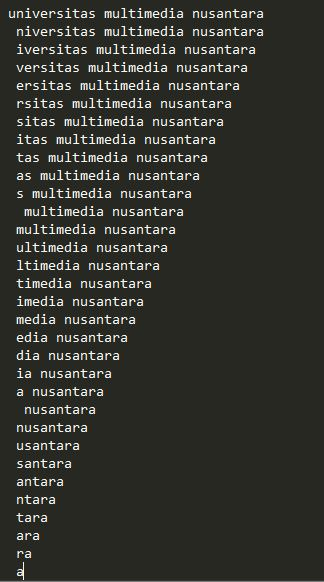
\includegraphics[width=1\textwidth]{plagiarisme/perulangan.JPG}}
	\caption{perulangan.}
	\label{perulangan}
	\end{plagiarisme}
Contoh diatas adalah perulangan yang menghilangkan satu karakter pertama sebuah string dengan menggunakan irisan while x.

Berikut ini satu lagi contoh untuk menampilkan bilangan genap kurang dari 11.
Python 2.4.3(#1,May 24 2008,13:47:28) [GGc 4.1.2 20070626 (Red Hat 4.1.2-14)] on linux2 Type "help", "copyright", "credits" or "license" for more information.
>>> x=0
>>> while x<10 :
... $x = x + 1$
... if x % 2:
...       continue
... else:
...       print x,
...
2 4 6 8 10
>>>
Beberapa bentuk for adalah sebagai berikut:
Perulangan sederhana
for x in range(0,10):
      print x,
perulangan di dalam perulangan
for x in range (0,10):
      for y in range (0,10):
              print y,
print x,
Perulangan dengan else
for x in range(0,10):
      print x,
else:
  print 'Perulangan sudah selesai'
 Hasilnya :
 Python 2.4.3(#1,May 24 2008, 13:47:28) [GCC 4.1.2 20070626 (Red Hat 4.1.2-14)] on linux2
 Type "help", "copyright", "credits" or "license" for more information.
 >>> for x in range(0,10):
 ... print x
 ...
 0 1 2 3 4 5 6 7 8 9
 >>>
 Python 2.4.3 (#1,May 24 2008, 13:47:28) [GCC 4.1.2 20070626 (Red Hat 4.1.2-14)] on linux2
 Type "help", "copyright", "credits" or "license" for more information.
 >>> for x in range(0,10):
 ... for y in range(0,10):
 ...       print y,
 ...
  0 1 2 3 4 5 6 7 8 9 0 1 2 3 4 5 6 7 8 9 0 1 2 3 4 5 6 7 8 9 
 0 1 2 3 4 5 6 7 8 9 0 1 2 3 4 5 6 7 8 9 0 1 2 3 4 5 6 7 8 9
 0 1 2 3 4 5 6 7 8 9 0 1 2 3 4 5 6 7 8 9 0 1 2 3 4 5 6 7 8 9
 0 1 2 3 4 5 6 7 8 9
 >>> print x,
 9
 
\subsection{Komputasi}
komputasi dengan bahasa: Statistik Sederhana
mari kita kembali ke eksplorasi kita tentang cara membawa sumber daya komputasi kita untuk menghasilkan teks dalam jumlah banyak.
Pada bagian ini, kita mengambil pertanyaan tentang apa yang membuat teks menjadi distinc, dan gunakan metode otomatis untuk menemukan kata-kata dan ekspresi teks yang khas.
Sebelum melanjutkan lebih lanjut, Anda mungkin ingin memeriksa pemahaman Anda tentang bagian terakhir dengan memprediksikan output dari kode berikut. Anda bisa menggunakan penerjemah untuk memeriksa apakah Anda benar. Jika Anda tidak yakin bagaimana melakukan tugas ini, sebaiknya Anda meninjau bagian sebelumnya sebelum melanjutkan lebih jauh.
>>> saying = ['After', 'all', 'is', 'said',  'and', 'done',
...                    'more', 'is','said', 'than', 'done']
>>> tokens = set(saying)
>>> tokens = sorted(tokens)
>>> tokens[ -2:]
what output do you expext here?
>>>

\subsection{fitur dan keunggulan python}
Beberapa fitur yang dapat dikatakan sebagai keunggulan python yaitu :
\begin{enumerate}
\item Python is powerful and fast, artinya python merupakan suatu kumpulan modul-modul yang sangat baik  dan dapat menangani secara praktis setiap domain masalah.
\item Python plays well with others, artinya python dapat beritegrasi dengan Component Object Model (COM), NET dan objek-objek Common Object Request Broker Architecture (COBRA).
\item Python runs everywhere, artinya python tersedia untuk berbagai macam sistem operasi seperti windows, unix atau linux, OS/2, mac, Amiga dll.
\item Python is friendly and easy to learn, artinya python sangat bersahabat bagi penggunanya.
\item Python is open, artinya python dibawah lisensi open source yang membuatnya dapat disebarkan secara bebas nbahkan untuk keperluan komersil.
\end{enumerate}

\subsection{Script Python}
    Seringkali pengguna harus menuliskan ekspresi yang cukup kompleks dan akan digunakan secara berulang di kemudian hari. Untuk keperluan penulisan ekspresi kompleks, kita dapat membuatnya dalam sebuah script yang dibantu dengan adanya teks editor. Penulis menggunakan vi teks editor default yang terdapat pada distro GNU/Linux. Pada contoh berikut ini, kita dapat melihat contoh script Python yang sederhana : 
vi contoh-script-01.py
#!/usr/bin/python
a = 1
print 'Nilai a adalah :',a
simpan script anda dengan :
:wq!
  Secara default, script Python yang anda buat akan disimpan dengan ekstensi .py . Anda dapat melakukan eksekusi script yang telah anda buat tersebut dengan cara :
    	python contoh-script-01.py
    atau :
    Memberikan permission x (executable) sehingga
   script tersebut dapat dijalankan, dengan perintah :
    chmod +x contoh-script-01.py
    /contoh-script-01.py

\subsection{Kelebihan dan Kekurangan}
\subsubsection{Kelebihan}
\begin{enumerate}
\item Tidak ada tahapan kompilasi dan penyambungan (link) sehingga kecepatan perubahan pada masa pembuatan sistem aplikasi meningkat.
\item Tidak ada deklarasi tipe data yang merumitkan sehingga program menjadi lebih sederhana, singkat, dan fleksible.
\item Manajemen memori otomatis yaitu kumpulan sampah memori sehingga dapat menghindari pencacatan kode.
\item Tipe data dan operasi tingkat tinggi yaitu kecepatan pembuatan sistem aplikasi menggunakan tipe objek yang telah ada.
\item Pemrograman berorientasi objek.
\item Pelekatan dan perluasan dalam C.
\item Terdapat kelas, modul, eksepsi sehingga terdapat dukungan pemrograman skala besar secara modular.
\item Pemuatan dinamis modul C sehingga ekstensi menjadi sederhana dan berkas biner yang kecil.
\item Pemuatan kembali secara dinamis modul phyton seperti memodifikasi aplikasi tanpa menghentikannya.
\item Model objek universal kelas Satu.
\item Konstruksi pada saat aplikasi berjalan.
\item Interaktif, dinamis dan alamiah.
\item Akses hingga informasi interpreter.
\item Portabilitas secara luas seperti pemrograman antar platform tanpa ports.
\item Kompilasi untuk portable kode byte sehingga kecepatan eksekusi bertambah dan melindungi kode sumber.
\item Antarmuka terpasang untuk pelayanan keluar seperti perangkat Bantu system, GUI, persistence, database, dll.
\end{enumerate}

\subsubsection{Kekurangan}
\begin{enumerate}
\item Beberapa penugasan terdapat diluar dari jangkauan python, seperti bahasa pemrograman dinamis lainnya, python tidak secepat atau efisien sebagai statis, tidak seperti bahasa pemrograman kompilasi seperti bahasa C.
\item Disebabkan python merupakan interpreter, python bukan merupakan perangkat bantu terbaik untuk pengantar komponen performa kritis.
\item Python tidak dapat digunakan sebagai dasar bahasa pemrograman implementasi untuk beberapa komponen, tetapi dapat bekerja dengan baik sebagai bagian depan skrip antarmuka untuk mereka.
\item Python memberikan efisiensi dan fleksibilitas tradeoff by dengan tidak memberikannya secara menyeluruh. Python menyediakan bahasa pemrograman optimasi untuk kegunaan, bersama dengan perangkat bantu yang dibutuhkan untuk diintegrasikan dengan bahasa pemrograman lainnya.
\item Banyak terdapat referensi lama terutama dari pencarian google, python adalah pemrograman yang sangat lambat. Namun belum lama ini ditemukan bahwa Google, Youtube, DropBox dan beberapa software sistem banyak menggunakan Python.
\item Kini Python menjadi salah satu bahasa pemrograman yang populer digunakan oleh pengembangan $  $web, aplikasi $  $web, aplikasi perkantoran, simulasi, dan masih banyak lagi. $  $ Hal ini disebabkan karena Python bahasa pemrograman yang dinamis dan mudah dipahami.
\item Selain itu, sekarang telah tersedia berbagai situs kursus yang bagus untuk mempelajari bahasa pemrograman Python ini sehingga pembaca maupun developer pemula yang akan mempelajari bahasa ini akan menjadi lebih mudah karena dapat berlatih dimanapun dan kapanpun selama terhubung dengan Internet.
\item Menariknya, berbagai situs kursus gratis ini menawarkan metode pembelajaran yang interaktif sehingga mudah dimengerti oleh pesertanya.
\end{enumerate}

\subsection{Elemen Dasar Python}
Bahasa pemrograman python memiliki beberapa elemen penting, diantaranya yaitu :
\begin{enumerate}
	\item Himpunan Karakter
		Semua karakter di python terdiri dari huruf besar, huruf kecil, angka dan simbol-simbol lainnya yang terdapat pada keyword dapat digunakan untuk menandai atau memberikan nama terhadap sebuah data atau object.
	\item Pengenal 
		Pengenal (identifier) merupakan suatu nama yang biasa dipakai oleh user (programmer) untuk menamakan : variabel, konstanta, tipe data, fungsi, label, objek, serta hal-hal lain. Karena python memiliki penamaan case sensitive maksudnya huruf besar dan kecil berbeda.Contoh : No_mahasiswa berbeda dengan no_mahasiswa
	\item Nama Variabel harus diawali dengan huruf atau karakter garis bawah (_), selanjutnya dapat diikuti dengan huruf maupun angka atau tanda garis bawah.Nama Variabel tidak boleh diawali dengan angka.
	\item Nama Variabel tidak boleh menggunakan operator-operator aritmatika dan karakter khusus.
	\item jika nama variabel terdiri dari dua atau lebih, maka antar kata tidak diperbolehkan menggunakan spasi
	\item Nama Variabel tidak boleh menggunakan kata-kata yang telah memiliki arti khusus dalam bahasa python.
	\item Penggunaan huruf kecil dan huruf besar dibedakan.
	\item Panjang maksimal suatu variabel adalah 32 karakter sehingga jika mendeklarasikan suatu variabel yang panjangnya lebih dari 32 karakter, secara otomatis sistem tetap akan mengenali sepanjang 32 karakter saja.
	\item Kata Kunci
		Kata kunci (keywords) merupakan pengenal ke sistem python yang mempunyai arti khusus bagi interpreter python dan kata kunci juga merupakan kumpulan kata yang dicadangkan. kata-kata ini tidak boleh digunakan sebagai identifier.
Pada gambar \ref{tabel} dijelaskan bahwa kata kunci sebagai berikut.
\begin{plagiarisme}[ht]
	\centerline{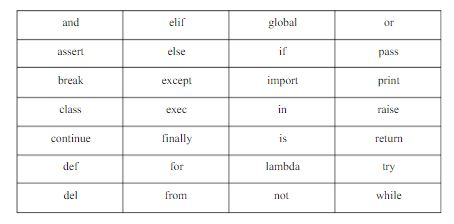
\includegraphics[width=1\textwidth]{plagiarisme/tabel.JPG}}
	\caption{tabel.}
	\label{tabel}
	\end{plagiarisme}
\end{enumerate}

\subsection {Nested Code Block}
Sebagian besar bahasa pemrograman mengizinkan kita untuk melakukan blok kode saat ekspresi bersyarat, atau jika pernyataan, dipuaskan.
Jika pernyataan memeriksa apakah tes len (kata) <5 itu benar. itu, jadi tubuh jika pernyataan dipanggil dan pernyataan cetak dijalankan, menampilkan pesan kepada pengguna. ingatlah untuk menjelaskan pernyataan cetak dengan mengetikkan empat spasi.
>>> kata = 'kucing'
>>> jika len (kata) <5:
... print 'word long kurang dari 5'
... 1
panjang kata kurang dari 5
Saat kita menggunakan penerjemah python kita harus menambahkan baris kosong tambahan 1 agar bisa mendeteksi bahwa blok yang disarangkan selesai.
